
\section{Getting started}\label{sec:start}\index{PISM!getting started}

We get started with an extended example.  It applies PISM to model the Greenland ice sheet using data assembled by the \href{http://websrv.cs.umt.edu/isis/index.php/SeaRISE_Assessment}{Sea-level Response to Ice Sheet Evolution (SeaRISE)} group \cite{Bindshadler2012SeaRISE}.  SeaRISE is a community-organized assessment process providing an upper bound on ice sheet contributions to sea level in the next 100--200 years, especially for the IPCC AR5 report in 2013.

The example in this section is a hands-on first look at PISM.  It is not an in-depth tutorial, and some details of what is happening will only be explained later.  Other sections list PISM options, discuss and help user's evaluate modeling choices, and explain the ways users will need to preprocess input data.

Some of the PISM output figures in this section were produced using a supercomputer.  But the basic run here can be done on a typical workstation or capable laptop.  That is why a rather coarse $20\,\textrm{km}$ grid is used in the main example in this section.  Of course PISM makes much higher spatial resolution possible by exploiting large-scale parallel processing.


To install PISM, see the Installation Manual at \href{http://www.pism-docs.org}{\texttt{www.pism-docs.org}}.
Once installed, executables \texttt{pismr} and \texttt{pclimate} should be available (i.e.~on your system's ``path''; confirm with ``\texttt{which pismr}'').  The instructions below also assume you are using a \texttt{bash} shell or one that accepts \texttt{bash} syntax.


\subsection{SeaRISE input data for the Greenland ice sheet}

The NetCDF data file which we use for input is freely-available online.  Descriptions of the data it contains, and a link to the file itself, are on this web page: 
\medskip

\centerline{\protect{\textbf{\url{http://websrv.cs.umt.edu/isis/index.php/Present_Day_Greenland}}}}
\medskip

\noindent The quickest way to get the file is to do
\begin{verbatim}
$ cd examples/searise-greenland
$ ./preprocess.sh
\end{verbatim}
\noindent The script \texttt{preprocess.sh}\footnote{\protect{This script requires \texttt{wget} and also NCO (NetCDF Operators; \url{http://nco.sourceforge.net/})}.} downloads the version 1.1 SeaRISE ``master'' present-day data set.  It adjusts the metadata in this file to make it PISM-readable.  In fact it creates several new NetCDF files which can be read by PISM; use \texttt{ncdump -h} to see their metadata.  Two of the new files contain famous time-dependent paleo-climate records from ice core and seabed core records; \texttt{pism_dT.nc} has GRIP while \texttt{pism_dSL.nc} has SPECMAP.

Also the preprocess script downloads the SeaRISE summary versions of IPCC AR4 (2007) climate projections, namely \texttt{ar4_precip_anomaly.nc} and \texttt{ar4_temp_anomaly.nc}.  These files are downloaded from \href{http://www.pism-docs.org/}{\texttt{www.pism-docs.org}}, but they are versions of the data at the SeaRISE page \url{http://websrv.cs.umt.edu/isis/index.php/Future_Climate_Data}.  These surface temperature and precipitation scenarios are used in the script \texttt{experiments.sh} to demonstrate offline coupling (forcing) in subsection \ref{subsect:forecastcaution} below.

Any of these NetCDF files can be viewed with \texttt{ncview} or other NetCDF visualization tools; see Table \ref{tab:NetCDFview} below.  An application of IDV to the master data set produced Figure \ref{fig:sr-input}, for example.

\begin{figure}[ht]
\centering
\mbox{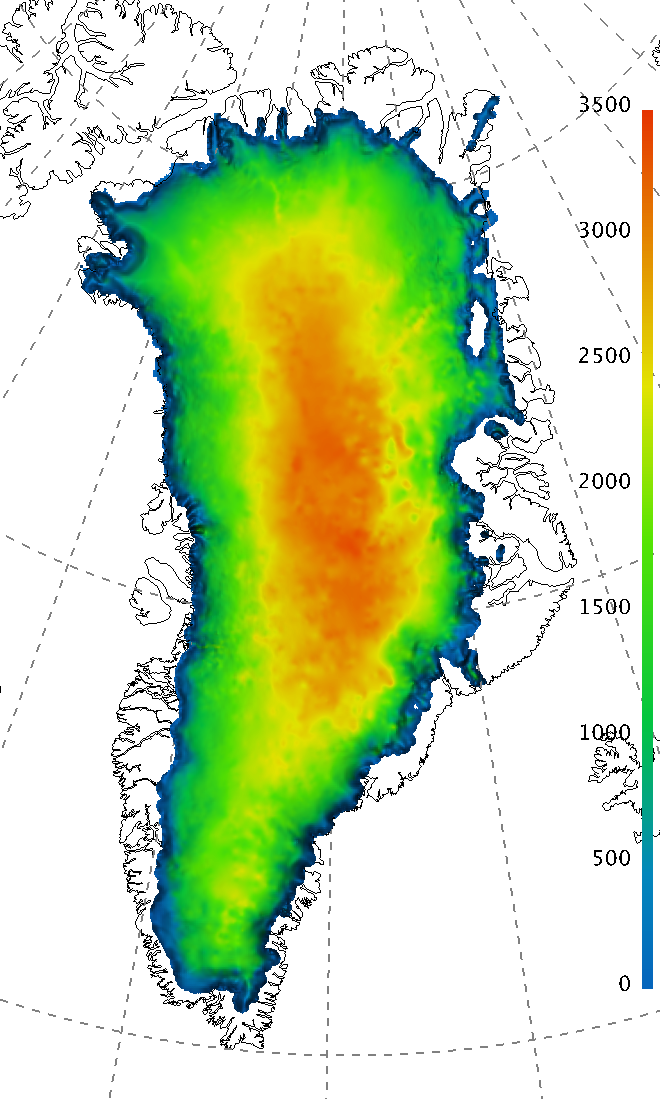
\includegraphics[width=2.0in,keepaspectratio=true]{sr-greenland-thk}
  \qquad
  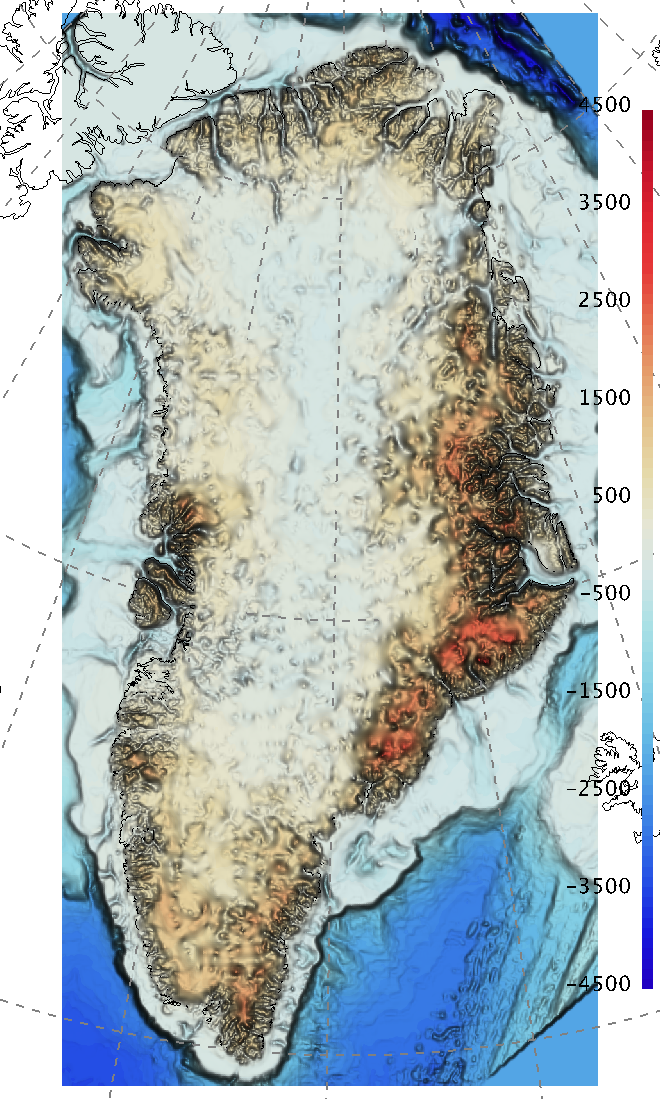
\includegraphics[width=2.0in,keepaspectratio=true]{sr-greenland-topg}
  \qquad
  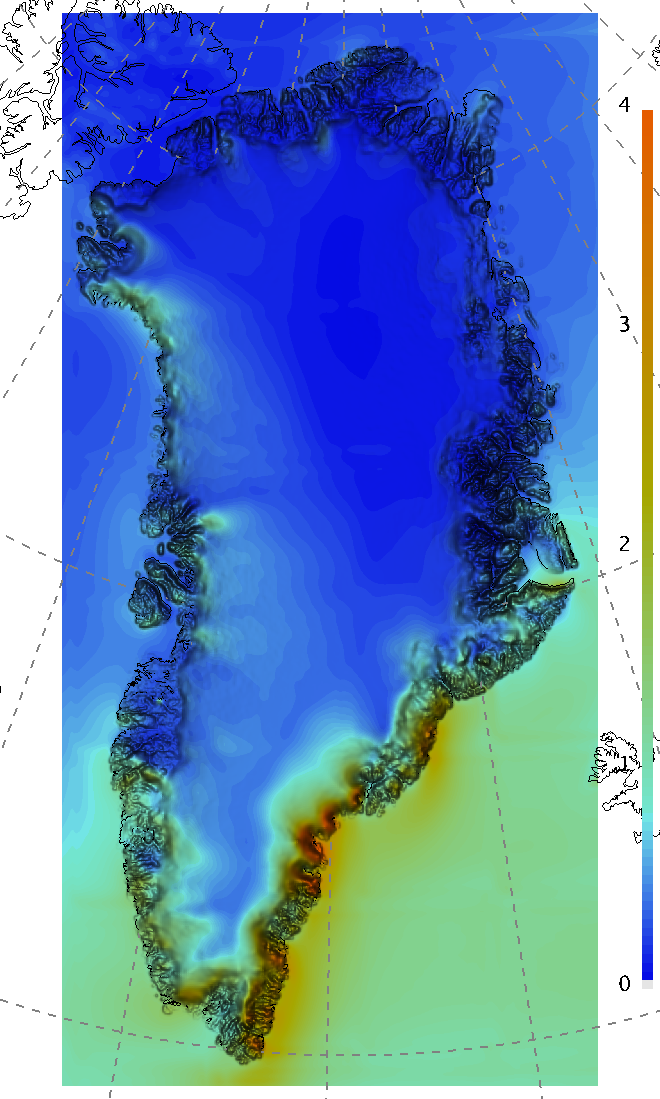
\includegraphics[width=2.0in,keepaspectratio=true]{sr-greenland-prcp}}
\caption{The input present-day ice thickness (left; m), bedrock elevation (center; m), and present-day precipitation (right; m $\text{a}^{-1}$ ice equivalent) for SeaRISE-Greenland.  These are fields \texttt{thk}, \texttt{topg}, and \texttt{precipitation}, respectively, in file \texttt{pism_Greenland_5km_v1.1.nc} produced by running \texttt{preprocess.sh}.}
\label{fig:sr-input}
\end{figure}


\subsection{Run PISM}   \label{subsect:runscript}  We are ready to run PISM.  Like many Unix programs, PISM allows many command-line options.  Furthermore there are configuration parameters that get read from a file---see \mbox{\texttt{src/pism_config.cdl}} in the PISM source code.  Because PISM handles many different ice sheet, shelf, and glacier configurations, the list of user-configurable flags and parameters is quite long; for a complete list see \url{\PISMBROWSERURL}.  Therefore in practice we often build scripts to run PISM with the correct options, and we have done this for \mbox{SeaRISE-Greenland}.

Modeling ice sheets can be done by integrating paleo-climatic and long-time-scale information to build a model for the present state of the ice sheet, so our main script is called ``\texttt{spinup.sh}''.  The spin-up stage is the one which generally requires the most processor-hours, compared to a follow-on ``forecast'' stage.  To see what is done during spin-up, do this:
\begin{verbatim}
$ PISM_DO=echo ./spinup.sh |less
\end{verbatim}
Setting the environment variable \texttt{PISM_DO} in this way tells \texttt{spinup.sh} just to print out the commands it is about to run, not do them.\footnote{The script outputs more than a page so we pipe to \texttt{less}.  If you don't have \texttt{less}, try \texttt{more}.}

Note that ``\texttt{mpiexec -n 2 pismr}'' appears in the PISM runs done by \texttt{spinup.sh}.  This means that, by default in this script, the PISM executable \texttt{pismr} is run in parallel on two processes (e.g.~cores).  The executable name ``\texttt{pismr}'' stands for the standard ``run'' mode of PISM, in contrast to other, specialized modes described later.

For the rest of this example, we assume you have a workstation with 8 cores, but this example will work with 1 to 500 processes, with good scaling in speed.  The script takes the number of processes as its first argument (illustrated below).

The script \texttt{spinup.sh} starts by ``bootstrapping.''  This term describes the creation, by heuristics and simplified models, of the kind of full initial conditions needed for the evolving, time-dependent ice dynamics model.  In fact the first 100 model year run commanded by \texttt{spinup.sh} is this:
\small
\begin{verbatim}
mpiexec -n 8 pismr -config_override searise_config.nc -climatic_mass_balance_cumulative \
  -skip -skip_max 10 -boot_file pism_Greenland_5km_v1.1.nc -Mx 76 -My 141 \
  -Lz 4000 -Lbz 2000 -Mz 101 -Mbz 11 -z_spacing equal \
  -atmosphere searise_greenland -surface pdd -ocean_kill \
  -y 100 -o g20km_pre100.nc
\end{verbatim}
\normalsize
The options describe a $76\times 141$ point grid in the horizontal, which gives 20 km grid spacing in both directions.  There are also important choices about the vertical extent and resolution of the computational grid; more on those later. 

Now, let's actually get the run going:
\begin{verbatim}
$ ./spinup.sh 8 >> out.spin20km &
\end{verbatim}
\noindent Because we have re-directed the text output, PISM will show what it is doing in the text file \texttt{out.spin20km} as it runs in the background.  Using \texttt{less} is a good way to watch such a growing text file.  Quickly the run will produce an early flow result in \texttt{g20km_pre100.nc}.

Soon after that some climatic boundary conditions sample results will appear in \texttt{g20km_climate-500a.nc}.  Such output from executable \texttt{pclimate} is effectively a movie of the stored and modeled climatic inputs provided to our ice dynamics model, including the results from surface models like the above-mentioned PDD model for surface mass balance.  This is a convenient way to, early in the modeling process, look at the critical surface mass balance and surface temperature inputs to the ice dynamics.


\subsection{Watching the spin-up}  \label{subsect:spinupsketch}  The next paragraphs describe what happens and what files are produced by the run which is underway.  We believe that the modeling choices represented here are reasonable, but they are not the only way to do it.  The user is encouraged to experiment; that is the point of a model!

After the completion of the first 100 model year run (\texttt{g20km_pre100.nc}), we then work to generate a more-physical enthalpy (i.e.~temperature and liquid fraction) field in which the modeled ice internal energy, its temperature, its softness, its stored basal water, and its basal melt rate are all in better balance with the ice sheet geometry and the simultaneously evolving flow velocity field.  Note the velocity advects the ice properties, especially enthalpy and thus ice softness.

The upper and lower surfaces of this modeled ice are held fixed at this stage.  The upper surface is held fixed by the option \texttt{-no_mass}, while the lower surface is held fixed in the sense that we do not yet apply a bed deformation model.  The resulting enthalpy field is in approximate equilibrium with a velocity field for which the surface kinematical equation \cite{Fowler} is unfortunately \emph{not} satisfied.  Also there is no sliding at this stage because good sliding requires good basal strength which requires good basal melt rates; these improve significantly as this no-sliding run evolves.

We sometimes call this early stage ``pre-spin-up'', a stage which follows on ``bootstrapping'' and comes before the classical paleo-climatic data-using ``spin-up''.  This ``pre-spin-up'' stage goes for 50,000 model years and yields the file \texttt{g20km_steady.nc} at the end.  Along the way the file \texttt{ex_g20km_steady.nc} is updated at every 500 model years, and it can be used to evaluate the degree to which we have reached a thermomechanically-coupled steady state.


\begin{figure}[ht]
\centering
%  temppabase from last time in ex_g10km_steady.nc and driving stress taud from g10km_SIA.nc
\mbox{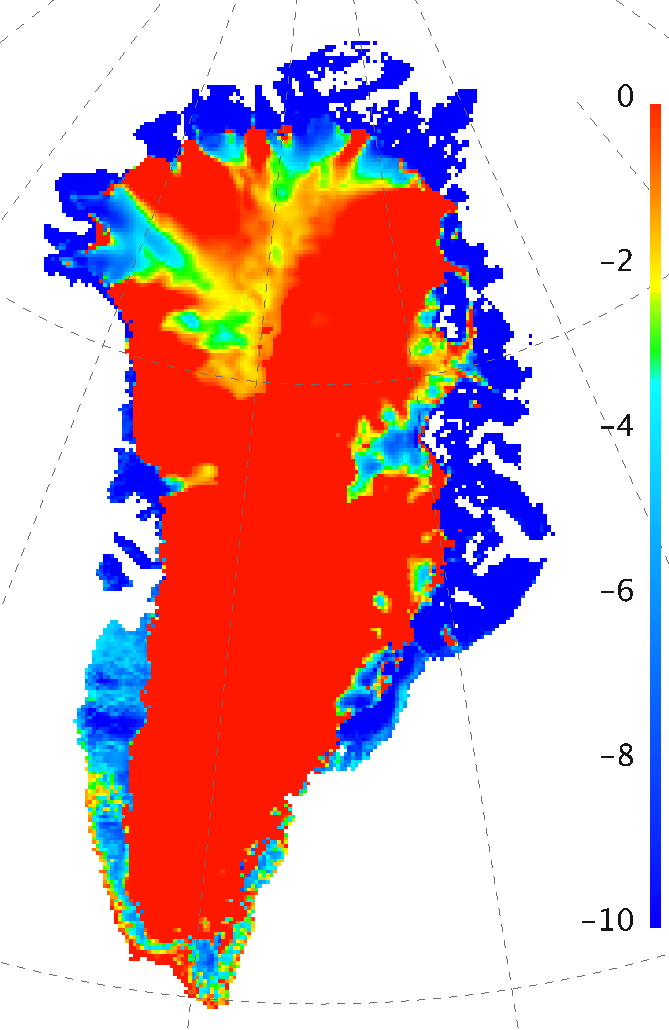
\includegraphics[width=2.0in,keepaspectratio=true]{temppabase}
  \qquad 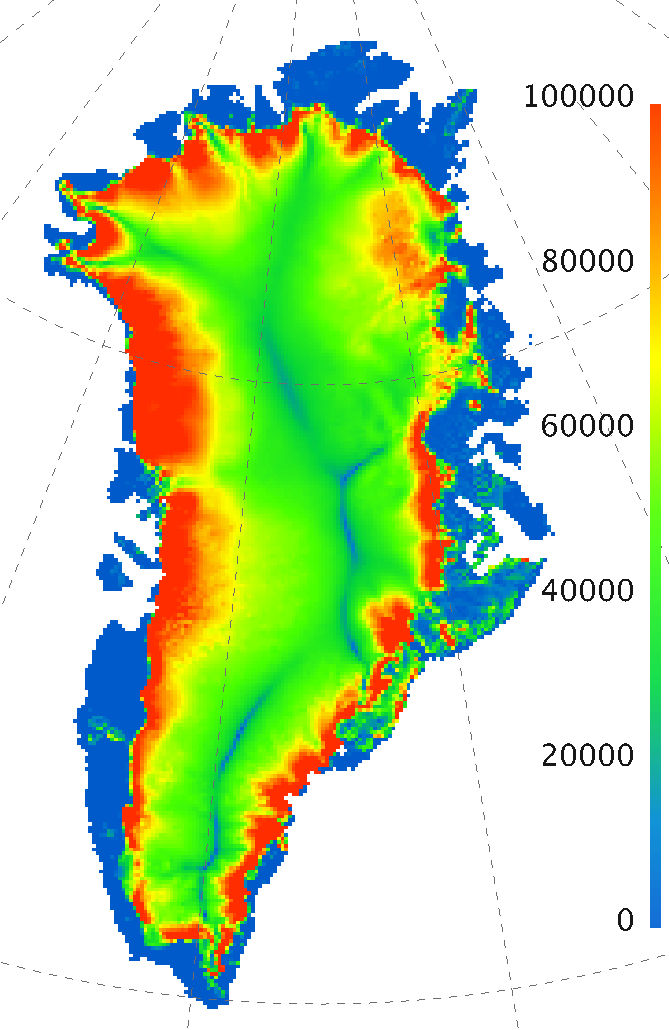
\includegraphics[width=2.1in,keepaspectratio=true]{taud}}
\caption{Part of the model state at the beginning of paleo-climate-modeling ice sheet spin-up, in file \texttt{g20km_steady.nc} from running \texttt{spinup.sh}.  Left: pressure-adjusted basal temperature ($\phantom{|}^\circ$C; field \texttt{temp_pa}).  Right: driving stress magnitude $\rho g H |\grad h|$ (Pa; field \texttt{taud_mag}).}
\label{fig:sr-spinstart}
\end{figure}

The resulting model state in \texttt{g20km_steady.nc} is our model for the state of the Greenland ice sheet at the beginning of the paleo-climate record provided in the SeaRISE data set, namely 125,000 B.P.  There is, obviously, great uncertainty in this model for the distant past of the Greenland ice sheet.  Two views of the 10\,km model grid version of this state are in Figure \ref{fig:sr-spinstart}.

\begin{figure}[ht]
\centering
%  thk, cbase, csurf from g10km_0.nc
\mbox{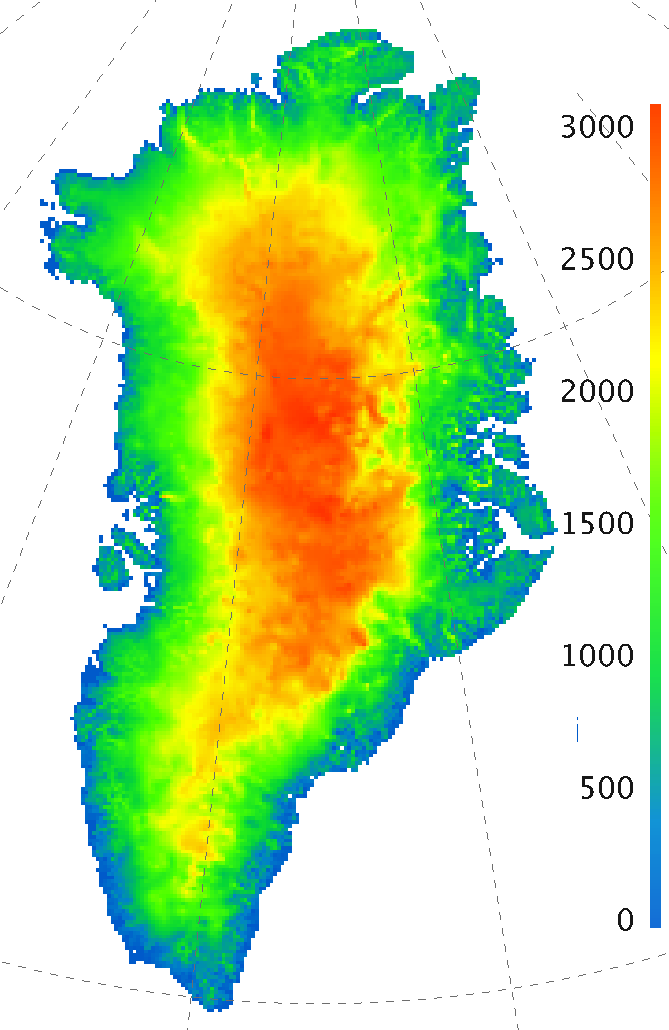
\includegraphics[width=2.in,keepaspectratio=true]{thk}
  \qquad 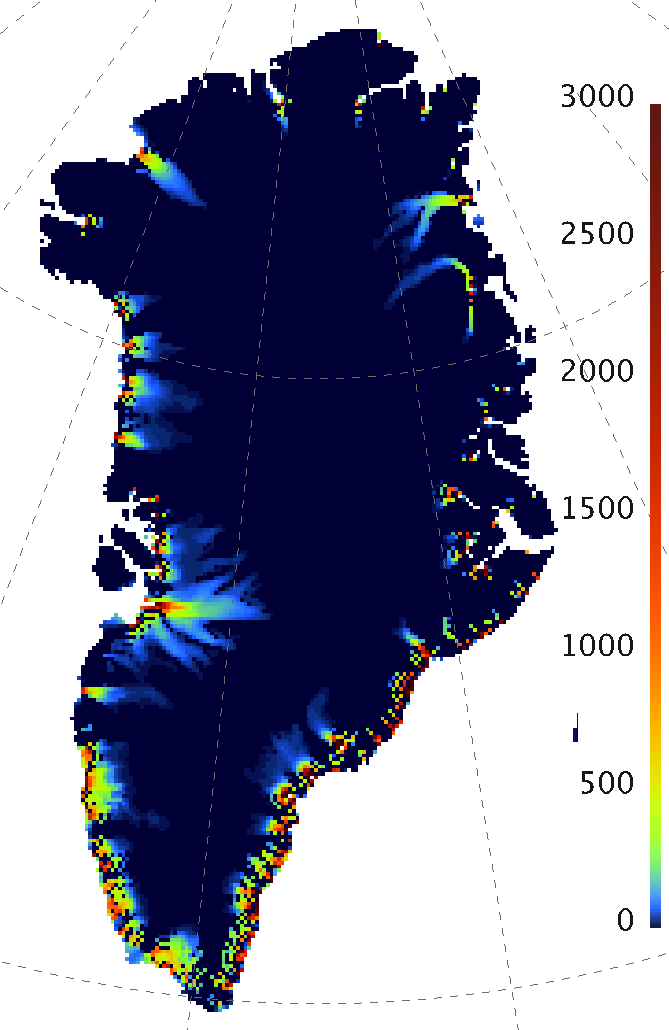
\includegraphics[width=2.in,keepaspectratio=true]{cbase}
  \qquad 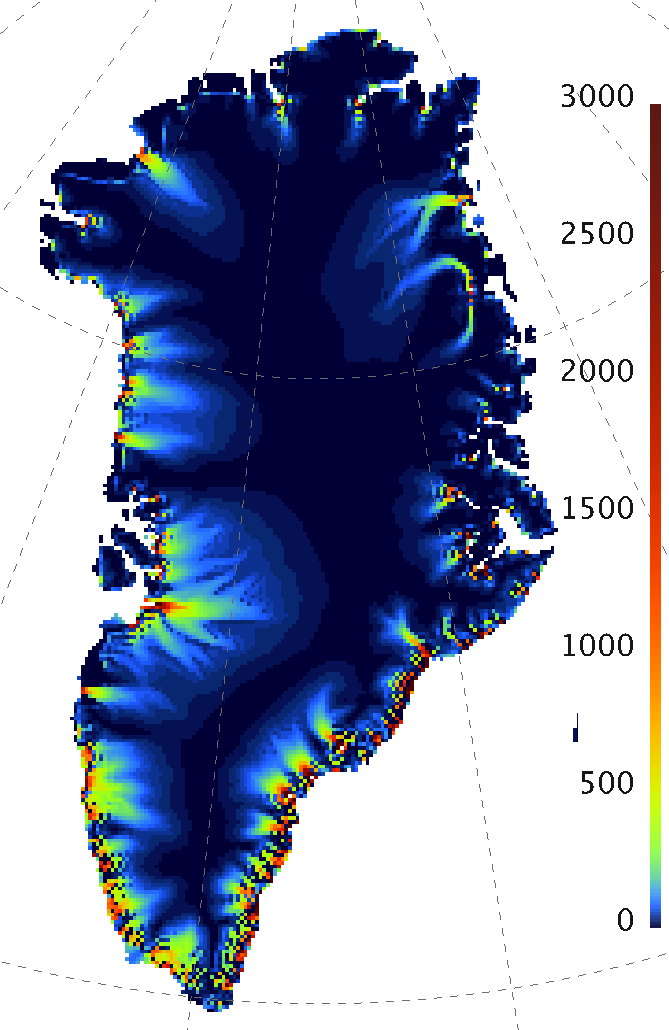
\includegraphics[width=2.in,keepaspectratio=true]{csurf}}
\caption{Model for the present-day Greenland ice sheet, based on spin-up over 125,000 model years using paleo-climate forcing.  Left: ice thickness (m).  Center: basal sliding speed (m/a).  Right: surface speed (m/a).  These are fields \texttt{thk}, \texttt{cbase}, and \texttt{csurf} from file \texttt{g10km_0.nc}.}
\label{fig:sr-spindone-map}
\end{figure}

The actual paleo-climate-driven spin-up starts from model state \texttt{g20km_steady.nc}.  We turn on three new mechanisms, climatic forcing, bed deformation, and improved stress balance.  There are two forms of climatic forcing. First, temperature offsets from GRIP core data affect the snow energy balance and thus rates of melting and runoff; the model is a simple temperature-index scheme described at the SeaRISE website.  Thereby the surface mass balance varies over time; in warm periods there is more marginal ablation.  Additionally, sea levels from the SPECMAP cores affects which ice is floating.

Significantly, we start using a more complete ice dynamics model with sliding controlled by a membrane stress balance, the SIA+SSA hybrid model described in section \ref{sec:dynamics}.  This is turned on with option ``\texttt{-ssa_sliding}''.  Also, we turn on a bed deformation model; the option is ``\texttt{-bed_def lc}''.  These options are discussed in section \ref{sec:modeling-choices}.  The command itself (do \verb|PISM_DO=echo ./spinup.sh 8| to see) is
\small
\begin{verbatim}
mpiexec -n 8 pismr -config_override searise_config.nc -climatic_mass_balance_cumulative \
  -skip -skip_max 10 -i g20km_steady.nc -ssa_sliding -thk_eff -topg_to_phi 5.0,20.0,-300.0,700.0 \
  -bed_def lc -atmosphere searise_greenland,delta_T -surface pdd -paleo_precip pism_dT.nc \
  -atmosphere_delta_T_file pism_dT.nc \
  -ocean constant,delta_SL -ocean_delta_SL_file pism_dSL.nc -ocean_kill pism_Greenland_5km_v1.1.nc \
  -ts_file ts_g20km_m5000a.nc -ts_times -125000:yearly:-5000 -extra_file ex_g20km_m5000a.nc \
  -extra_vars ... -extra_times -125000:500:-5000 -ys -125000 -ye -5000 -o g20km_m5000a.nc
\end{verbatim}
\normalsize
but where the full list \verb|-extra_vars| is suppressed.  It uses option \verb|-i| for its input file \verb|g20km_steady.nc|, which is a PISM output file containing the grid information; contrast this with the earlier run which had options \verb|-boot_file| and specified a grid.   (A grid specification uses options \verb|-Mx|, \verb|-My|, \verb|-Mz|, etc.; see subsection \ref{subsect:grid}.)  This run command illustrates that PISM allows a great deal of command-line control, which is a desirable feature, but it also means in practice that most PISM modeling is done using shell scripts to run executables, as here.

This run goes from the SeaRISE-Greenland start time of -125,000 years to -5,000 years.  In this period, diagnostic outputs are written into \texttt{ex_g20km_m5000a.nc} at every 500 model years, and scalar time series including total ice volume are written into \texttt{ts_g20km_m5000a.nc} at every model year.  At the end of this period of the spinup we get the model state file \texttt{g20km_m5000a.nc}.  After that, a final run continues on the same grid from -5,000 years to present day, producing \texttt{g20km_0.nc}.  A variation on this last 5,000 model years run is put in \texttt{g20km_0_ftt.nc}.



The spun-up states \texttt{g20km_0.nc} or \texttt{g20km_0_ftt.nc} is intended to be a model for the Greenland ice sheet at the present day, and thus a basis on which to explore future ice sheet behavior.  If you run \texttt{./spinup N 2} then all of this is done on a 10\,km grid.  Figure \ref{fig:sr-spindone-map} shows some fields from the 10\,km model grid version of this present-day state.  The ice sheet thickness and surface velocity can be compared to present-day observations \cite{BKAJS}, and parameter dependences in the spin-up process should be explored.

Over the course of the spin-up we have saved the modeled ice volume in ``time-series'' NetCDF files.  This important model output can be viewed by
\begin{verbatim}
$ ncview ts_g20km_m5000a.nc ts_g20km_0.nc
\end{verbatim}
\noindent Figure \ref{fig:sr-spindone-ivolboth} shows this ice volume time series for the whole spin-up.  We see the modeled volatility of ice volume in the late ``Eemian'' period, between -120,000 and -115,000 BPE in the SeaRISE version of the GRIP temperature data.  We also see that the result \emph{does} depend on resolution.  Higher resolution grids allow the model to better resolve the flux through outlet glaciers especially, which are topographically-controlled, and such an effect explains the greater Eemian volume loss in the above 10\,km time series.  See the later examples in this manual for more on high resolution modeling.

\begin{figure}[ht]
\centering
\includegraphics[width=4.5in,keepaspectratio=true]{ivolboth}
\caption{Time series of modeled ice sheet volume on 20km and 10km grids.}
\label{fig:sr-spindone-ivolboth}
\end{figure}

%from PISM0.4:  On an 8 core workstation the total run time for the complete 20\,km spin-up, which models 125,000 model years with ``full physics'' of the polythermal SIA+SSA hybrid type (section \ref{sec:dynamics}) is about 5 wall clock hours or 40 processor-hours.  For the same machine, the complete 10\,km spin-up used about 660 processor-hours, thus several wall-clock days.

On an the total run time for the complete 20\,km spin-up, which models 125,000 model years with ``full physics'' of the polythermal SIA+SSA hybrid type (section \ref{sec:dynamics}) is about 290 processor-hours.  The complete 10\,km spin-up used about 6131 processor-hours.

If done without membrane stresses (i.e.~non-sliding SIA only) these computational times are significantly reduced.  The polythermal versus ``cold'' energy-conservation choice corresponds to no performance difference of consequence.


\subsection{Going forward}  \label{subsect:forecastcaution}  In the same \verb|examples/searise-greenland| directory is a script \verb|experiments.sh|.  This does a suite of runs for 500 years into the future for the SeaRISE assessment, initializing from the above-computed modeled present-day state.  The first run is a ``control''  run assuming steady climate for the entire period.  Other runs perform the experiments described at \url{http://websrv.cs.umt.edu/isis/index.php/Category_1:_Whole_Ice_Sheet}.  Some runs use the AR4 climate forcing files which were produced when you ran \texttt{preprocess.sh}.  Once these runs are completed there are postprocessing scripts which primarily adjust metadata to match the standardizations used for the SeaRISE assessment.

Please run \verb|experiments.sh| and the postprocessing scripts, play with them, and modify them, but remember that we include these scripts for demonstration purposes.

Because real ice sheets, and ice sheet models too, have a ``memory'' of past climates, the results strongly depend on the nature of the spin-up process which preceded this ``forecast'' run.  Therefore, as already noted, it is critical to evaluate the quality of the spunup state, for example using present-day observations of surface velocity \cite{AschwandenAdalgeirsdottirKhroulev}, and other observations including ice temperature in ice bore-holes.  Critical thinking about a broad range of modeling hypotheses is prerequisite to building models of future behavior.


\subsection{Handling NetCDF files}\label{subsect:nctoolsintro}  At a superficial level, PISM is just a program which takes one or more NetCDF files as input, does some computation, and produces one or more NetCDF files as output.  As a result, the user needs tools to extract some meaning from the NetCDF output files and also, in the general case, more tools to create NetCDF files for input to PISM.\footnote{Regarding the creation of input files, see the section \ref{sec:bootstrapping-format} and table \ref{tab:modelhierarchy} for ideas about the data necessary for modeling.}

The most basic tools for converting NetCDF files to and from a standard text representation are called \texttt{ncdump} and \texttt{ncgen}.  A glance at Unix \texttt{man} pages for these tools might be wise at this time.

We most-regularly use \texttt{ncview} to look at NetCDF files.  Table \ref{tab:NetCDFview} lists NetCDF tools that can be useful for visualizing and post-processing PISM output files, as well as for preparing input data.  We find \texttt{ncview}, NCO, IDV and PyNGL especially useful.

\newcommand{\netcdftool}[1]{#1\index{NetCDF!tools!#1}}
\begin{table}[ht]
\centering
\small
\begin{tabular}{llp{0.4\linewidth}}
  \toprule
  \textbf{Tool} & \textbf{Site} & \textbf{Function} \\
  \midrule
  \netcdftool{\texttt{ncdump}} & \emph{included with any NetCDF distribution} & dump binary NetCDF as \texttt{.cdl} (text) file \\
  \netcdftool{\texttt{ncgen}} & \emph{included with any NetCDF distribution} & convert \texttt{.cdl} file to binary NetCDF \\
  \netcdftool{\texttt{ncview}} & \href{http://meteora.ucsd.edu/~pierce/ncview_home_page.html}{\texttt{meteora.ucsd.edu/~pierce/ncview_home_page.html}} & quick graphical view \\
  \netcdftool{IDV} & \url{http://www.unidata.ucar.edu/software/idv/} & more complete visualization \\
  % \netcdftool{Paraview} & \href{http://www.paraview.org}{\texttt{www.paraview.org}} & powerful open-source parallel visualization \\
  \netcdftool{NCL} &  \url{http://www.ncl.ucar.edu} & NCAR Command Language\\
  \netcdftool{PyNGL} &  \url{http://www.pyngl.ucar.edu} & Python version of NCL\\
  % \netcdftool{VisIt} & \href{http://visit.llnl.gov}{\texttt{visit.llnl.gov}} & advanced parallel visualization \\
  \netcdftool{NCO}\index{NCO (NetCDF Operators)} & \url{http://nco.sourceforge.net/} & NetCDF Operators; command-line tools\\
  \netcdftool{CDO} & \url{http://code.zmaw.de/projects/cdo} & Climate Data Operators; more command-line tools, including conservative re-mapping \\
  & \url{www.unidata.ucar.edu/software/netcdf/} & root for NetCDF information \\
  \bottomrule
\end{tabular}
\normalsize
\caption{Tools for viewing and modifying NetCDF files.}
\label{tab:NetCDFview}
\end{table}


%%% Local Variables: 
%%% mode: latex
%%% TeX-master: "manual"
%%% End: 


% LocalWords:  metadata SPECMAP paleo html IDV
